\documentclass[9pt]{beamer}  % Default is 11pt
\usetheme{Madrid}
\usecolortheme{default}
\usepackage[utf8]{inputenc}
\usepackage{amsmath}
\usepackage{amsfonts}
\usepackage{amssymb}
\usepackage{tikz}
\usepackage{xcolor}
\usepackage{hyperref}
\usepackage{graphicx}
\title{CRISC Exam - Hard Concepts \& Exam Traps}
\subtitle{Section 2: IT Risk Assessment Deep Dive Tutorial}
\author{CRISC Mastery Series}
\date{\today}

\begin{document}
	
	% ============================================================
	% TITLE SLIDE
	% ============================================================
\begin{frame}
	\fontsize{3}{4}\selectfont
	\titlepage
\end{frame}
	% ============================================================
	% OUTLINE
	% ============================================================
\begin{frame}[shrink]{Section 2 Tutorial Outline}


	\tableofcontents
\end{frame}
	
	% ============================================================
	% SECTION 1: RISK MANAGEMENT LIFE CYCLE
	% ============================================================
	\section{1. Risk Management Life Cycle}
	
	% ----------------------------------------------------------------------
	\subsection{1.1 The 5-Step Life Cycle}
	\begin{frame}{1.1 The IT Risk Management Life Cycle}
		\begin{center}
			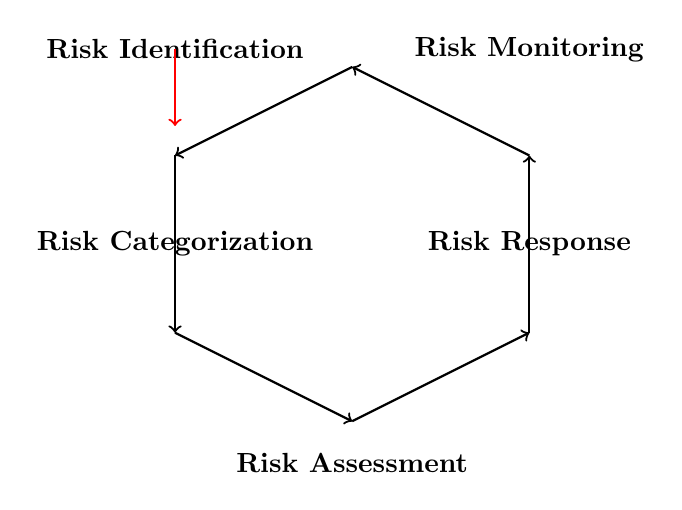
\begin{tikzpicture}[scale=0.75]
				% Draw cycle
				\draw[thick, ->] (0,0) -- (0,-3);
				\draw[thick, ->] (0,-3) -- (3,-4.5);
				\draw[thick, ->] (3,-4.5) -- (6,-3);
				\draw[thick, ->] (6,-3) -- (6,0);
				\draw[thick, ->] (6,0) -- (3,1.5);
				\draw[thick, ->] (3,1.5) -- (0,0);
				
				% Labels
				\node at (0,1.8) {\textbf{Risk Identification}};
				\node at (0,-1.5) {\textbf{Risk Categorization}};
				\node at (3,-5.2) {\textbf{Risk Assessment}};
				\node at (6,-1.5) {\textbf{Risk Response}};
				\node at (6,1.8) {\textbf{Risk Monitoring}};
				
				% Arrows showing continuous cycle
				\draw[->, thick, red] (0,1.8) -- (0,0.5);
			\end{tikzpicture}
		\end{center}
	\end{frame}
	
	\begin{frame}{1.1 Detailed Life Cycle}
		\begin{block}{Step 1: Risk Identification}
			\begin{itemize}
				\item \textbf{First} step - "You can't protect what you don't know"
				\item Identify all \textbf{threats} and \textbf{vulnerabilities}
				\item Document in \textbf{risk register}
				\item \textbf{Iterative} process - risks emerge over time
			\end{itemize}
		\end{block}
		
		\begin{block}{Step 2: Risk Categorization}
			\begin{itemize}
				\item Classify risks by \textbf{type} and \textbf{severity}
				\item Critical/High/Medium/Low
				\item Assign to appropriate stakeholders
				\item Enables \textbf{prioritization}
			\end{itemize}
		\end{block}
		
		\begin{alertblock}{The Critical Trap}
			Risk identification is \textbf{NOT} a one-time event. New risks emerge throughout the project/organizational life cycle!
		\end{alertblock}
	\end{frame}
	
	\begin{frame}{1.1 Steps 3-5}
		\begin{block}{Step 3: Risk Assessment}
			\begin{itemize}
				\item Evaluate based on \textbf{likelihood} and \textbf{impact}
				\item Determine \textbf{risk score} (Likelihood × Impact)
				\item Compare against \textbf{risk appetite} and \textbf{tolerance}
				\item Prioritize risks for treatment
			\end{itemize}
		\end{block}
		
		\begin{block}{Step 4: Risk Response}
			\begin{itemize}
				\item Select treatment strategy: \textbf{Mitigate, Accept, Transfer, Avoid}
				\item Implement \textbf{controls}
				\item Document in \textbf{risk register}
				\item Obtain \textbf{management approval}
			\end{itemize}
		\end{block}
		
		\begin{block}{Step 5: Risk Monitoring}
			\begin{itemize}
				\item \textbf{Continuous} monitoring of risks and controls
				\item Track \textbf{KRIs} and \textbf{KPIs}
				\item Identify \textbf{emerging risks}
				\item Review \textbf{control effectiveness}
			\end{itemize}
		\end{block}
	\end{frame}
	
	% ----------------------------------------------------------------------
	\subsection{1.2 Issues, Events, Incidents, Breaches}
	\begin{frame}{1.2 Critical Terminology - The Hierarchy}
		\begin{block}{Understanding the Progression}
			\begin{center}
				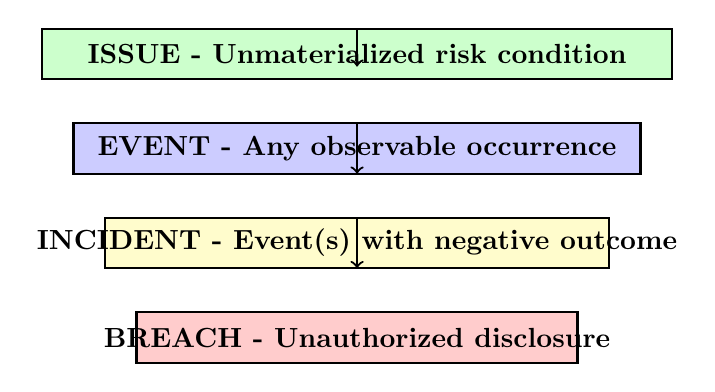
\begin{tikzpicture}[scale=0.8]
					\draw[thick, fill=green!20] (0,0) rectangle (10,0.8) node[midway] {\textbf{ISSUE - Unmaterialized risk condition}};
					\draw[thick, fill=blue!20] (0.5,-1.5) rectangle (9.5,-0.7) node[midway] {\textbf{EVENT - Any observable occurrence}};
					\draw[thick, fill=yellow!20] (1,-3) rectangle (9,-2.2) node[midway] {\textbf{INCIDENT - Event(s) with negative outcome}};
					\draw[thick, fill=red!20] (1.5,-4.5) rectangle (8.5,-3.7) node[midway] {\textbf{BREACH - Unauthorized disclosure}};
					
					\draw[->, thick] (5,0.8) -- (5,0.2);
					\draw[->, thick] (5,-0.7) -- (5,-1.5);
					\draw[->, thick] (5,-2.2) -- (5,-3);
				\end{tikzpicture}
			\end{center}
		\end{block}
		
		\begin{alertblock}{The Critical Trap}
			These terms are \textbf{NOT} interchangeable! Each represents a different level of severity and requires different responses.
		\end{alertblock}
	\end{frame}
	
	\begin{frame}{1.2 Detailed Definitions}
		\begin{block}{Issues}
			\begin{itemize}
				\item Instance of IT risk that has \textbf{NOT materialized}
				\item Needs to be considered and kept on the \textbf{radar}
				\item Combination of control, value, and threat conditions
				\item \textbf{Example}: Outdated operating systems being used by employees
			\end{itemize}
		\end{block}
		
		\begin{block}{Events}
			\begin{itemize}
				\item Any \textbf{observable} occurrence during a period of time
				\item Three types: Threat event, Loss event, Vulnerability event
				\item \textbf{Example}: A single failed login attempt
			\end{itemize}
		\end{block}
	\end{frame}
	
	\begin{frame}{1.2 Incidents and Breaches}
		\begin{block}{Incidents}
			\begin{itemize}
				\item Event or \textbf{combination of events} with \textbf{negative outcome}
				\item Affects \textbf{CIA triad}
				\item Requires \textbf{immediate response}
				\item \textbf{Example}: Thousands of failed login attempts in one second
			\end{itemize}
		\end{block}
		
		\begin{block}{Breaches}
			\begin{itemize}
				\item \textbf{Accidental} or \textbf{unlawful} destruction, loss, alteration
				\item Unauthorized \textbf{disclosure} or \textbf{access}
				\item \textbf{Regulatory} reporting required
				\item \textbf{Example}: Yahoo breach (2016), Equifax breach (2017)
			\end{itemize}
		\end{block}
		
		\begin{exampleblock}{Key Distinction}
			\centering
			\textbf{Event} = Any occurrence \\
			\textbf{Incident} = Event(s) with \textit{negative} outcome \\
			\textbf{Breach} = Incident involving \textit{unauthorized} access/disclosure
		\end{exampleblock}
	\end{frame}
	
	% ============================================================
	% SECTION 2: THREAT, VULNERABILITY, AND RISK
	% ============================================================
	\section{2. Threat, Vulnerability, and Risk}
	
	% ----------------------------------------------------------------------
	\subsection{2.1 Core Concepts}
	\begin{frame}{2.1 The Threat-Vulnerability-Risk Relationship}
		\begin{center}
			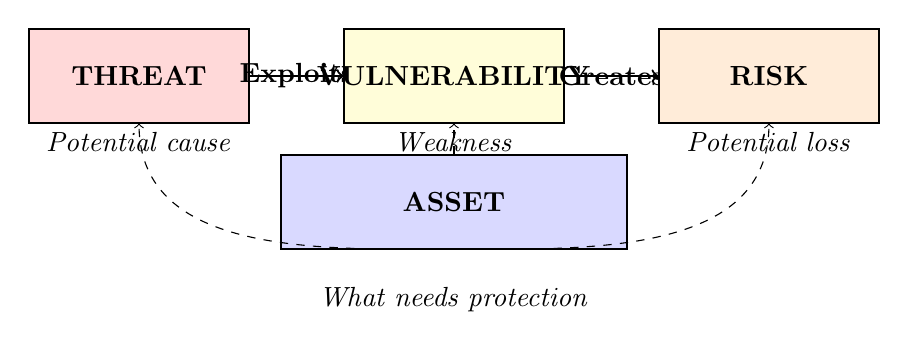
\begin{tikzpicture}[scale=0.8]
				% Threat box
				\draw[thick, fill=red!15] (0,0) rectangle (3.5,1.5) node[midway] {\textbf{THREAT}};
				\node at (1.75,-0.3) {\textit{Potential cause}};
				
				% Arrow to vulnerability
				\draw[->, thick] (3.5,0.75) -- (5,0.75) node[midway] {\textbf{Exploits}};
				
				% Vulnerability box
				\draw[thick, fill=yellow!15] (5,0) rectangle (8.5,1.5) node[midway] {\textbf{VULNERABILITY}};
				\node at (6.75,-0.3) {\textit{Weakness}};
				
				% Arrow to risk
				\draw[->, thick] (8.5,0.75) -- (10,0.75) node[midway] {\textbf{Creates}};
				
				% Risk box
				\draw[thick, fill=orange!15] (10,0) rectangle (13.5,1.5) node[midway] {\textbf{RISK}};
				\node at (11.75,-0.3) {\textit{Potential loss}};
				
				% Asset below
				\draw[thick, fill=blue!15] (4,-2) rectangle (9.5,-0.5) node[midway] {\textbf{ASSET}};
				\node at (6.75,-2.8) {\textit{What needs protection}};
				
				% Arrows from asset
				\draw[->, dashed] (6.75,-0.5) -- (6.75,0);
				\draw[->, dashed] (6.75,-2) to[out=180,in=270] (1.75,0);
				\draw[->, dashed] (6.75,-2) to[out=0,in=270] (11.75,0);
			\end{tikzpicture}
		\end{center}
		
		\begin{exampleblock}{The Formula}
			\centering
			\Large{\textbf{Risk = Threat × Vulnerability × Asset Value}}
		\end{exampleblock}
	\end{frame}
	
	\begin{frame}{2.1 Understanding Each Component}
		\begin{block}{Threat}
			\begin{itemize}
				\item Anything that could \textbf{impact} an asset
				\item Can be human, malicious code, natural disaster, etc.
				\item \textbf{Threat actor}: The entity that executes the threat
				\item \textbf{Threat vector}: The path used to gain access
			\end{itemize}
		\end{block}
		
		\begin{block}{Vulnerability}
			\begin{itemize}
				\item \textbf{Weakness} in design, implementation, or operation
				\item Can be exploited by a threat
				\item Exists in hardware, software, configuration, or processes
				\item \textbf{Can be controlled} by implementing safeguards
			\end{itemize}
		\end{block}
		
		\begin{block}{Risk}
			\begin{itemize}
				\item What happens when a threat exploits a vulnerability
				\item Potential \textbf{harm} to assets
				\item \textbf{Can be managed} but never eliminated
			\end{itemize}
		\end{block}
	\end{frame}
	
	\begin{frame}{2.1 Example - Malware Attack}
		\begin{block}{Scenario: Malware Infection}
			\begin{itemize}
				\item \textbf{Threat}: Malicious actor who wrote the malware
				\item \textbf{Threat Actor}: Hacker sending phishing emails
				\item \textbf{Threat Vector}: Phishing email with malicious attachment
				\item \textbf{Vulnerability}: Missing antivirus; user opened infected file
				\item \textbf{Risk}: Laptops infected; data compromised
				\item \textbf{Asset}: Company data and systems
			\end{itemize}
		\end{block}
		
		\begin{alertblock}{The Critical Insight}
			\begin{itemize}
				\item \textbf{Threats} are \textbf{NOT} within our control
				\item \textbf{Vulnerabilities} \textbf{CAN} be controlled
				\item \textbf{Risk} is the \textbf{result} of threat exploiting vulnerability
			\end{itemize}
		\end{alertblock}
	\end{frame}
	
	% ----------------------------------------------------------------------
	\subsection{2.2 Threat Modeling}
	\begin{frame}{2.2 Understanding Threat Modeling}
		\begin{block}{What is Threat Modeling?}
			\begin{itemize}
				\item \textbf{Structured approach} to identifying threats
				\item Identifies potential \textbf{vulnerabilities}
				\item Defines \textbf{security requirements}
				\item Quantifies threat criticality
				\item Prioritizes \textbf{remediation}
			\end{itemize}
		\end{block}
		
		\begin{block}{The 4-Step Cycle}
			\begin{enumerate}
				\item \textbf{Model}: "What are we building?"
				\item \textbf{Identify Threats}: "What could go wrong?"
				\item \textbf{Mitigate}: "What countermeasures do we have?"
				\item \textbf{Validate}: "Have we done all the steps?"
			\end{enumerate}
		\end{block}
	\end{frame}
	
	\begin{frame}{2.2 Threat Modeling Methods}
		\begin{block}{STRIDE}
			\begin{tabular}{|p{2.5cm}|p{4cm}|p{4.5cm}|}
				\hline
				\textbf{Threat} & \textbf{Description} & \textbf{Security Principle} \\
				\hline
				Spoofing & Impersonating another & Authenticity \\
				\hline
				Tampering & Modifying data & Integrity \\
				\hline
				Repudiation & Denying actions & Non-repudiation \\
				\hline
				Information Disclosure & Exposing data & Confidentiality \\
				\hline
				Denial of Service & Disrupting service & Availability \\
				\hline
				Elevation of Privilege & Gaining extra rights & Authorization \\
				\hline
			\end{tabular}
		\end{block}
	\end{frame}
	
	\begin{frame}{2.2 DREAD Model}
		\begin{block}{DREAD Risk Assessment}
			\begin{tabular}{|p{2.5cm}|p{8.5cm}|}
				\hline
				\textbf{Factor} & \textbf{Question} \\
				\hline
				\textbf{D}amage & How bad is an attack? \\
				\hline
				\textbf{R}eproducibility & How easy is it to reproduce? \\
				\hline
				\textbf{E}xploitability & What effort is required? \\
				\hline
				\textbf{A}ffected Users & How many people impacted? \\
				\hline
				\textbf{D}iscoverability & How easy is it to find? \\
				\hline
			\end{tabular}
		\end{block}
		
		\begin{block}{OCTAVE}
			\begin{itemize}
				\item \textbf{Operationally Critical Threat, Asset, and Vulnerability Evaluation}
				\item Focuses on \textbf{organizational risks}
				\item Self-directed methodology
				\item Business and IT teams work together
			\end{itemize}
		\end{block}
	\end{frame}
	
	% ----------------------------------------------------------------------
	\subsection{2.3 Vulnerability Analysis}
	\begin{frame}{2.3 Sources of Vulnerabilities}
		\begin{block}{Key Vulnerability Sources}
			\begin{itemize}
				\item \textbf{Vulnerability Assessment Scans} - Nessus, Qualys
				\item \textbf{Penetration Tests} - Annual or after major changes
				\item \textbf{Static Analysis} - Code pipeline issues
				\item \textbf{Dynamic Analysis} - Runtime scanning
				\item \textbf{Configuration Checks} - Misconfiguration issues
				\item \textbf{Risk Assessments} - Non-technical risks
				\item \textbf{Zero-Day Findings} - New vulnerabilities with no patch
				\item \textbf{Industry Advisories} - NIST, CISA, vendor bulletins
			\end{itemize}
		\end{block}
		
		\begin{exampleblock}{Key Insight}
			Identifying vulnerabilities is only half the battle. \textbf{Prioritizing and fixing} them is the other half!
		\end{exampleblock}
	\end{frame}
	
	\begin{frame}{2.3 Common Vulnerability Scoring System}
		\begin{block}{CVSS - Quantifying Vulnerabilities}
			\begin{itemize}
				\item \textbf{Industry standard} for scoring vulnerabilities
				\item Scores range from 0.0 to 10.0
				\item \textbf{Critical}: 9.0 - 10.0 - \textit{Immediate action required}
				\item \textbf{High}: 7.0 - 8.9 - \textit{Prioritize remediation}
				\item \textbf{Medium}: 4.0 - 6.9 - \textit{Address in normal cycle}
				\item \textbf{Low}: 0.1 - 3.9 - \textit{Consider for future}
			\end{itemize}
		\end{block}
		
		\begin{alertblock}{The Critical Trap}
			\textbf{NOT} all vulnerabilities are equal!
			\begin{itemize}
				\item Critical vulnerabilities must be remediated \textbf{IMMEDIATELY}
				\item Low vulnerabilities may be \textbf{accepted} or deferred
				\item Prioritization is \textbf{ESSENTIAL}
			\end{itemize}
		\end{alertblock}
	\end{frame}
	
	% ============================================================
	% SECTION 3: RISK ASSESSMENT APPROACHES
	% ============================================================
	\section{3. Risk Assessment Approaches}
	
	% ----------------------------------------------------------------------
	\subsection{3.1 Top-Down vs Bottom-Up}
	\begin{frame}{3.1 Top-Down vs Bottom-Up Assessment}
		\begin{center}
			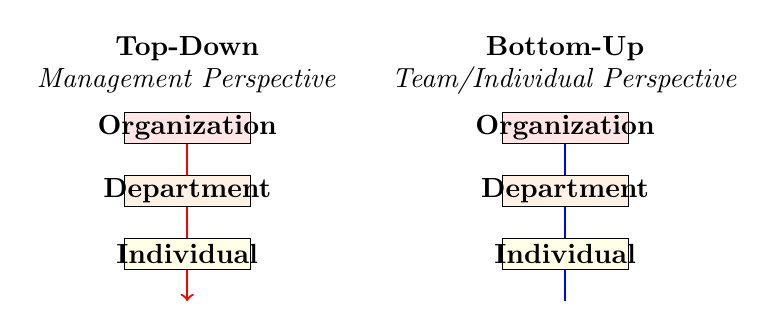
\begin{tikzpicture}[scale=0.8]
				% Top-down arrow
				\draw[->, thick, red] (2,1.5) -- (2,-1.5);
				\node at (2,2.5) {\textbf{Top-Down}};
				\node at (2,2.0) {\textit{Management Perspective}};
				
				% Bottom-up arrow
				\draw[->, thick, blue] (8,-1.5) -- (8,1.5);
				\node at (8,2.5) {\textbf{Bottom-Up}};
				\node at (8,2.0) {\textit{Team/Individual Perspective}};
				
				% Organization level
				\draw[fill=red!10] (1,1.5) rectangle (3,1.0) node[midway] {\textbf{Organization}};
				
				% Department level
				\draw[fill=orange!10] (1,0.5) rectangle (3,0) node[midway] {\textbf{Department}};
				
				% Individual level
				\draw[fill=yellow!10] (1,-0.5) rectangle (3,-1.0) node[midway] {\textbf{Individual}};
				
				% Bottom-up boxes
				\draw[fill=yellow!10] (7,-0.5) rectangle (9,-1.0) node[midway] {\textbf{Individual}};
				\draw[fill=orange!10] (7,0.5) rectangle (9,0) node[midway] {\textbf{Department}};
				\draw[fill=red!10] (7,1.5) rectangle (9,1.0) node[midway] {\textbf{Organization}};
			\end{tikzpicture}
		\end{center}
		
		\begin{block}{Which is Better?}
			\centering
			\Large{\textbf{Use BOTH approaches together!}}
		\end{block}
	\end{frame}
	
	\begin{frame}{3.1 Top-Down Assessment}
		\begin{block}{Characteristics}
			\begin{itemize}
				\item \textbf{Driven by} management perspective
				\item Related directly to \textbf{business objectives}
				\item Easier to get \textbf{buy-in}
				\item Results tend to be \textbf{broader} in nature
				\item Based on management's \textbf{experience} across multiple functions
			\end{itemize}
		\end{block}
		
		\begin{block}{Example: Healthcare EHR System}
			\begin{itemize}
				\item Board considers \textbf{strategic risks} with revenue implications
				\item E\&C reviews \textbf{regulatory risks}
				\item Senior management evaluates \textbf{departmental risks}
				\item Cyber reports inform \textbf{system-specific risks}
			\end{itemize}
		\end{block}
	\end{frame}
	
	\begin{frame}{3.1 Bottom-Up Assessment}
		\begin{block}{Characteristics}
			\begin{itemize}
				\item Identified by \textbf{individuals and teams}
				\item Cascaded up to department and organization level
				\item More \textbf{catered to specific business functions}
				\item Raised by \textbf{subject matter experts}
				\item Provides \textbf{detailed operational insights}
			\end{itemize}
		\end{block}
		
		\begin{block}{Example: Healthcare EHR System}
			\begin{itemize}
				\item System-level components analyzed first
				\item Individual departments assess operational impact
				\item Senior management understands \textbf{KPI impacts}
				\item Organizational level considers \textbf{regulatory} and \textbf{reputational} risks
			\end{itemize}
		\end{block}
	\end{frame}
	
	% ----------------------------------------------------------------------
	\subsection{3.2 Qualitative vs Quantitative}
	\begin{frame}{3.2 Qualitative Risk Analysis}
		\begin{block}{Characteristics}
			\begin{itemize}
				\item Based on \textbf{subjective} parameters
				\item Uses: High, Medium, Low, Very Low
				\item Assigns values based on \textbf{experience and expertise}
				\item \textbf{Less expensive}
				\item \textbf{Quick} to perform
				\item May be \textbf{biased} based on team expertise
			\end{itemize}
		\end{block}
		
		\begin{block}{Example}
			\begin{itemize}
				\item Likelihood: High/Medium/Low
				\item Impact: High/Medium/Low
				\item Risk Score: Likelihood × Impact (e.g., High × High = Critical)
			\end{itemize}
		\end{block}
	\end{frame}
	
	\begin{frame}{3.2 Quantitative Risk Analysis}
		\begin{block}{Characteristics}
			\begin{itemize}
				\item Based on \textbf{monetary values}
				\item Uses \textbf{historical data} for modeling
				\item Requires \textbf{reasonably accurate} data
				\item \textbf{More expensive}
				\item \textbf{Complex}; may need additional tools
				\item Results are \textbf{data-driven}
			\end{itemize}
		\end{block}
		
		\begin{block}{Key Formulas}
			\begin{itemize}
				\item \textbf{SLE} = AV × EF
				\begin{itemize}
					\item SLE = Single Loss Expectancy
					\item AV = Asset Value
					\item EF = Exposure Factor (\% loss)
				\end{itemize}
				\item \textbf{ALE} = SLE × ARO
				\begin{itemize}
					\item ALE = Annualized Loss Expectancy
					\item ARO = Annualized Rate of Occurrence
				\end{itemize}
			\end{itemize}
		\end{block}
	\end{frame}
	
	\begin{frame}{3.2 Quantitative Examples}
		\begin{block}{SLE Calculation Example}
			\begin{itemize}
				\item Asset Value = \$125,000
				\item Exposure Factor = 25\% (0.25)
				\item SLE = \$125,000 × 0.25 = \textbf{\$31,250}
			\end{itemize}
		\end{block}
		
		\begin{block}{ALE Calculation Example}
			\begin{itemize}
				\item SLE = \$31,250
				\item ARO = 4 (expected to happen 4 times per year)
				\item ALE = \$31,250 × 4 = \textbf{\$125,000}
			\end{itemize}
		\end{block}
		
		\begin{alertblock}{The Critical Trap}
			\begin{itemize}
				\item \textbf{Quantitative} is more complex and costlier
				\item \textbf{Qualitative} is subjective but faster
				\item \textbf{Choose based on business need}, not sophistication
			\end{itemize}
		\end{alertblock}
	\end{frame}
	
	\begin{frame}{3.2 Comparison Table}
		\begin{block}{Qualitative vs Quantitative}
			\begin{tabular}{|p{4.5cm}|p{5.5cm}|}
				\hline
				\textbf{Qualitative} & \textbf{Quantitative} \\
				\hline
				Subjective & Objective \\
				\hline
				Risk severity is important & Monetary value is important \\
				\hline
				Requires experience and expertise & Requires historical data and modeling \\
				\hline
				Relatively straightforward & Complex \\
				\hline
				Results can be biased & Results are data-driven \\
				\hline
				Less expensive & More expensive \\
				\hline
			\end{tabular}
		\end{block}
		
		\begin{exampleblock}{Semiquantitative (Hybrid)}
			\begin{itemize}
				\item Combines \textbf{both} approaches
				\item Assigns numerical values to qualitative ratings
				\item Example: High = 5, Medium = 3, Low = 1
				\item Risk Score = Likelihood Score × Impact Score
			\end{itemize}
		\end{exampleblock}
	\end{frame}
	
	% ============================================================
	% SECTION 4: RISK ASSESSMENT FRAMEWORKS
	% ============================================================
	\section{4. Risk Assessment Frameworks}
	
	% ----------------------------------------------------------------------
	\subsection{4.1 Industry Frameworks}
	\begin{frame}{4.1 Risk Assessment Frameworks}
		\begin{block}{Common Frameworks}
			\begin{tabular}{|p{2.5cm}|p{4cm}|p{4.5cm}|}
				\hline
				\textbf{Framework} & \textbf{Description} & \textbf{Best For} \\
				\hline
				NIST SP 800-30 & Risk management for general IS & General organizations \\
				\hline
				NIST SP 800-37 & Risk management for federal IS & Government agencies \\
				\hline
				NIST SP 800-161 & Supply chain risk management & Supply chain \\
				\hline
				ISO/IEC 27005 & Information security risk & IS risk management \\
				\hline
				ISO/IEC 31000 & Organizational risk & Enterprise risk \\
				\hline
				FAIR & Quantitative risk taxonomy & Quantitative analysis \\
				\hline
				OCTAVE & Asset-based risk & Enterprise IT projects \\
				\hline
			\end{tabular}
		\end{block}
	\end{frame}
	
	\begin{frame}{4.1 Choosing the Right Framework}
		\begin{block}{Considerations}
			\begin{itemize}
				\item \textbf{Industry} requirements
				\item \textbf{Regulatory} compliance needs
				\item \textbf{Organizational} maturity
				\item \textbf{Available} resources
				\item \textbf{Budget} constraints
				\item \textbf{Culture} and risk appetite
			\end{itemize}
		\end{block}
		
		\begin{exampleblock}{Key Insight}
			\begin{itemize}
				\item No single framework fits all organizations
				\item Choose what \textbf{makes sense} for your organization
				\item \textbf{Mix and match} frameworks if needed
				\item Ensure framework aligns with \textbf{business objectives}
			\end{itemize}
		\end{exampleblock}
	\end{frame}
	
	% ----------------------------------------------------------------------
	\subsection{4.2 Risk Assessment Techniques}
	\begin{frame}{4.2 Common Risk Assessment Techniques}
		\begin{block}{Technique Overview}
			\begin{tabular}{|p{2.5cm}|p{4cm}|p{4.5cm}|}
				\hline
				\textbf{Technique} & \textbf{Type} & \textbf{Description} \\
				\hline
				Bayesian Analysis & Quantitative & Uses prior data for probability \\
				\hline
				Bow Tie Analysis (BTA) & Diagram-based & Shows causes, controls, consequences \\
				\hline
				Brainstorming & Qualitative & Generates ideas with group \\
				\hline
				Delphi Method & Qualitative & Anonymous expert consensus \\
				\hline
				Event Tree Analysis & Quantitative & Forward-looking probabilities \\
				\hline
				Fault Tree Analysis & Quantitative & Top-down event analysis \\
				\hline
				Monte Carlo Analysis & Quantitative & Repeated random sampling \\
				\hline
				SWOT Analysis & Qualitative & Strengths, Weaknesses, Opportunities, Threats \\
				\hline
			\end{tabular}
		\end{block}
	\end{frame}
	
	\begin{frame}{4.2 Key Techniques Explained}
		\begin{block}{Delphi Method}
			\begin{itemize}
				\item Uses \textbf{expert opinion}
				\item \textbf{Multiple rounds} of questionnaires
				\item Anonymous responses
				\item Builds \textbf{consensus}
				\item Prevents \textbf{undue influence}
			\end{itemize}
		\end{block}
		
		\begin{block}{Fault Tree Analysis (FTA)}
			\begin{itemize}
				\item Starts with an \textbf{event}
				\item \textbf{Top-down} analysis
				\item Examines possible means for event to occur
				\item Displays results in a \textbf{logical tree} diagram
				\item Identifies \textbf{root causes}
			\end{itemize}
		\end{block}
	\end{frame}
	
	\begin{frame}{4.2 Monte Carlo and FAIR}
		\begin{block}{Monte Carlo Analysis}
			\begin{itemize}
				\item \textbf{Quantitative} technique
				\item Uses \textbf{repeated random sampling}
				\item Establishes \textbf{aggregate variation}
				\item Inputs have defined distributions
				\item Results show \textbf{probability ranges}
			\end{itemize}
		\end{block}
		
		\begin{block}{Factor Analysis of Information Risk (FAIR)}
			\begin{itemize}
				\item \textbf{Quantitative} taxonomy
				\item Focuses on \textbf{data loss} events
				\item Establishes \textbf{accurate probabilities}
				\item Uses \textbf{frequency} and \textbf{magnitude}
				\item Industry standard for quantitative risk
			\end{itemize}
		\end{block}
	\end{frame}
	
	% ============================================================
	% SECTION 5: BUSINESS IMPACT ANALYSIS
	% ============================================================
	\section{5. Business Impact Analysis (BIA)}
	
	% ----------------------------------------------------------------------
	\subsection{5.1 BIA vs Risk Assessment}
	\begin{frame}{5.1 BIA vs Risk Assessment}
		\begin{block}{BIA (Business Impact Analysis)}
			\begin{itemize}
				\item Identifies \textbf{critical business processes}
				\item Assesses \textbf{impact of disaster}
				\item Determines \textbf{recovery priorities}
				\item Output: RPO, RTO, MTD
				\item \textbf{Primary Goal}: Show how quickly to recover
			\end{itemize}
		\end{block}
		
		\begin{block}{Risk Assessment}
			\begin{itemize}
				\item Identifies \textbf{threats} and \textbf{vulnerabilities}
				\item Evaluates \textbf{likelihood} and \textbf{impact}
				\item Recommends \textbf{controls}
				\item Output: Risk register, mitigation plans
				\item \textbf{Primary Goal}: Identify and manage threats
			\end{itemize}
		\end{block}
		
		\begin{alertblock}{The Critical Trap}
			BIA and Risk Assessment are \textbf{NOT} the same! \\
			\textbf{BIA} = "How quickly must we recover?" \\
			\textbf{Risk Assessment} = "What threats do we face?"
		\end{alertblock}
	\end{frame}
	
	% ----------------------------------------------------------------------
	\subsection{5.2 Recovery Objectives}
	\begin{frame}{5.2 Recovery Objectives}
		\begin{block}{Three Key Metrics}
			\begin{tabular}{|p{2.5cm}|p{4cm}|p{4.5cm}|}
				\hline
				\textbf{Metric} & \textbf{Definition} & \textbf{Direction} \\
				\hline
				\textbf{RPO} & Maximum acceptable data loss & \textbf{Backward-looking} \\
				\hline
				\textbf{RTO} & Maximum acceptable downtime & \textbf{Forward-looking} \\
				\hline
				\textbf{MTD} & Maximum tolerated outage & Total threshold \\
				\hline
			\end{tabular}
		\end{block}
		
		\begin{alertblock}{The Critical Trap}
			\begin{itemize}
				\item \textbf{RPO} = "How much data can we lose?" - \textbf{BACKWARD}
				\item \textbf{RTO} = "How long can we be down?" - \textbf{FORWARD}
				\item \textbf{NEVER} confuse RPO and RTO directions!
			\end{itemize}
		\end{alertblock}
	\end{frame}
	
	\begin{frame}{5.2 Recovery Objectives Example}
		\begin{block}{Scenario: Application Recovery}
			\begin{itemize}
				\item RPO = 4 hours
				\begin{itemize}
					\item Can accept losing up to 4 hours of data
					\item Backups must run at least every 4 hours
				\end{itemize}
				\item RTO = 8 hours
				\begin{itemize}
					\item Application must be restored within 8 hours
					\item Need plan for 8-hour recovery window
				\end{itemize}
				\item MTD = 12 hours
				\begin{itemize}
					\item Business cannot survive beyond 12 hours of downtime
					\item \textbf{RTO < MTD} must ALWAYS be true!
				\end{itemize}
			\end{itemize}
		\end{block}
		
		\begin{exampleblock}{Key Relationship}
			\centering
			\Large{\textbf{RTO must ALWAYS be less than MTD!}}
		\end{exampleblock}
	\end{frame}
	
	\begin{frame}{5.2 The Recovery Timeline}
		\begin{center}
			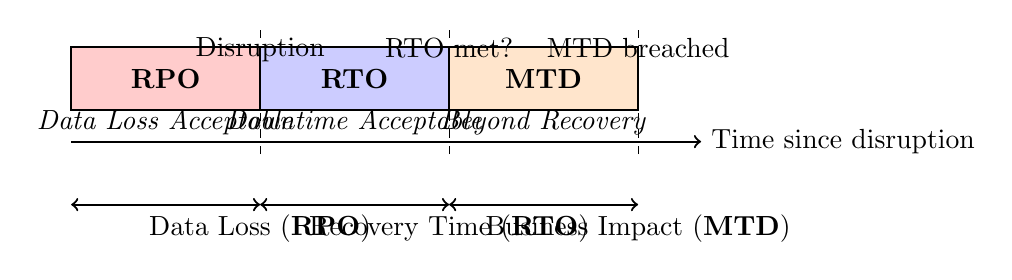
\begin{tikzpicture}[scale=0.8]
				% Timeline
				\draw[->, thick] (0,0) -- (10,0) node[right] {Time since disruption};
				
				% RPO area
				\draw[thick, fill=red!20] (0,0.5) -- (3,0.5) -- (3,1.5) -- (0,1.5) -- cycle;
				\node at (1.5,1.0) {\textbf{RPO}};
				\node at (1.5,0.3) {\textit{Data Loss Acceptable}};
				
				% RTO area
				\draw[thick, fill=blue!20] (3,0.5) -- (6,0.5) -- (6,1.5) -- (3,1.5) -- cycle;
				\node at (4.5,1.0) {\textbf{RTO}};
				\node at (4.5,0.3) {\textit{Downtime Acceptable}};
				
				% MTD area
				\draw[thick, fill=orange!20] (6,0.5) -- (9,0.5) -- (9,1.5) -- (6,1.5) -- cycle;
				\node at (7.5,1.0) {\textbf{MTD}};
				\node at (7.5,0.3) {\textit{Beyond Recovery}};
				
				% Dashed lines
				\draw[dashed] (3,-0.2) -- (3,1.8) node[below] {Disruption};
				\draw[dashed] (6,-0.2) -- (6,1.8) node[below] {RTO met?};
				\draw[dashed] (9,-0.2) -- (9,1.8) node[below] {MTD breached};
				
				% Arrows at bottom
				\draw[<->, thick] (0,-1) -- (3,-1) node[below] {Data Loss (\textbf{RPO})};
				\draw[<->, thick] (3,-1) -- (6,-1) node[below] {Recovery Time (\textbf{RTO})};
				\draw[<->, thick] (6,-1) -- (9,-1) node[below] {Business Impact (\textbf{MTD})};
			\end{tikzpicture}
		\end{center}
	\end{frame}
	
	% ============================================================
	% SECTION 6: INHERENT, RESIDUAL, AND CURRENT RISK
	% ============================================================
	\section{6. Inherent, Residual, and Current Risk}
	
	% ----------------------------------------------------------------------
	\subsection{6.1 Understanding the Risk Types}
	\begin{frame}{6.1 The Three Risk States}
		\begin{block}{Risk Types Defined}
			\begin{tabular}{|p{2.5cm}|p{4cm}|p{4.5cm}|}
				\hline
				\textbf{Risk Type} & \textbf{Definition} & \textbf{When Measured} \\
				\hline
				\textbf{Inherent Risk} & Risk \textbf{without} controls & Before any controls \\
				\hline
				\textbf{Residual Risk} & Risk \textbf{after} controls & After controls implemented \\
				\hline
				\textbf{Current Risk} & Risk in \textbf{real-time} & At specific point in time \\
				\hline
			\end{tabular}
		\end{block}
		
		\begin{alertblock}{The Critical Trap}
			\begin{itemize}
				\item \textbf{Residual} = Theoretical risk after controls
				\item \textbf{Current} = Real-time risk in actual environment
				\item They are \textbf{NOT} interchangeable!
			\end{itemize}
		\end{alertblock}
	\end{frame}
	
	\begin{frame}{6.1 The Risk Reduction Equation}
		\begin{center}
			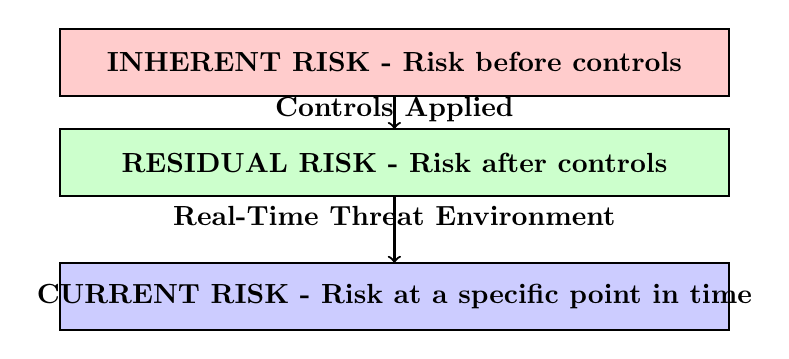
\begin{tikzpicture}[scale=0.85]
				% Inherent risk
				\draw[thick, fill=red!20] (0,0) rectangle (10,1) node[midway] {\textbf{INHERENT RISK - Risk before controls}};
				
				% Arrow down
				\draw[->, thick] (5,0) -- (5,-0.5);
				\node at (5,-0.2) {\textbf{Controls Applied}};
				
				% Residual risk
				\draw[thick, fill=green!20] (0,-1.5) rectangle (10,-0.5) node[midway] {\textbf{RESIDUAL RISK - Risk after controls}};
				
				% Arrow from residual to current
				\draw[->, thick] (5,-1.5) -- (5,-2.5);
				\node at (5,-1.8) {\textbf{Real-Time Threat Environment}};
				
				% Current risk
				\draw[thick, fill=blue!20] (0,-3.5) rectangle (10,-2.5) node[midway] {\textbf{CURRENT RISK - Risk at a specific point in time}};
			\end{tikzpicture}
		\end{center}
		
		\begin{exampleblock}{Key Formula}
			\centering
			\Large{\textbf{Residual Risk = Inherent Risk - Controls}}
		\end{exampleblock}
	\end{frame}
	
	\begin{frame}{6.1 Example - Laptop Security}
		\begin{block}{Scenario: Laptop Without Antivirus}
			\begin{itemize}
				\item \textbf{Inherent Risk}: Very high - laptop exposed to all viruses
				\item \textbf{Control}: Install antivirus software
				\item \textbf{Residual Risk}: Lower - protected against known viruses
				\item \textbf{Current Risk}: Varies daily - depends on new threats
			\end{itemize}
		\end{block}
		
		\begin{block}{Key Insights}
			\begin{itemize}
				\item \textbf{Inherent risk} is ever-present
				\item \textbf{Controls reduce} risk but never eliminate it
				\item \textbf{Residual risk} is what remains after controls
				\item \textbf{Current risk} changes with the threat landscape
			\end{itemize}
		\end{block}
	\end{frame}
	
	% ============================================================
	% SECTION 7: RISK REGISTER
	% ============================================================
	\section{7. Risk Register}
	
	% ----------------------------------------------------------------------
	\subsection{7.1 Understanding the Risk Register}
	\begin{frame}{7.1 What is a Risk Register?}
		\begin{block}{Definition}
			\begin{itemize}
				\item \textbf{Main reference} for all risk-related information
				\item Documents \textbf{all identified risks}
				\item Tracks \textbf{risk status} and \textbf{response}
				\item Supports \textbf{risk-related decisions}
			\end{itemize}
		\end{block}
		
		\begin{block}{Key Components}
			\begin{itemize}
				\item Risk \textbf{description}
				\item \textbf{Probability} of occurrence
				\item \textbf{Impact} if materialized
				\item \textbf{Risk Score} (Probability × Impact)
				\item \textbf{Inherent risk} level
				\item \textbf{Current controls}
				\item \textbf{Residual risk} level
				\item \textbf{Mitigation actions}
				\item \textbf{Risk owner}
				\item \textbf{Status} (Open/Closed/Monitoring)
			\end{itemize}
		\end{block}
	\end{frame}
	
	\begin{frame}{7.1 The Value of a Risk Register}
		\begin{alertblock}{The Critical Trap}
			\textbf{Common Mistake}: Thinking a risk register is just an inventory.
			
			\textbf{Correct}: A risk register drives risk response decisions and establishes accountability!
		\end{alertblock}
		
		\begin{block}{Primary Value}
			\begin{itemize}
				\item Drives the \textbf{risk response plan}
				\item Supports \textbf{prioritization} of responses
				\item Establishes \textbf{accountability}
				\item \textbf{Tracks} risk status over time
				\item Enables \textbf{reporting} and \textbf{dashboards}
			\end{itemize}
		\end{block}
	\end{frame}
	
	\begin{frame}{7.1 Risk Register Maintenance}
		\begin{block}{Best Practices}
			\begin{itemize}
				\item Update \textbf{continuously}, not just annually
				\item Review \textbf{at least quarterly}
				\item Assign \textbf{clear ownership}
				\item Link to \textbf{business objectives}
				\item Include \textbf{actionable} information
				\item Use \textbf{centralized} system with workflow
			\end{itemize}
		\end{block}
		
		\begin{alertblock}{The Critical Trap}
			\begin{itemize}
				\item \textbf{Annual updates} = Risk register is \textbf{outdated}
				\item Risk environment changes \textbf{constantly}
				\item Update \textbf{when risks change}, not on a fixed schedule
				\item \textbf{Regular} evaluation is needed (e.g., quarterly)
			\end{itemize}
		\end{alertblock}
	\end{frame}
	
	% ============================================================
	% SECTION 8: COMMON EXAM TRAPS
	% ============================================================
	\section{8. Common Exam Traps}
	
	% ----------------------------------------------------------------------
	\subsection{8.1 Risk Assessment Traps}
	\begin{frame}{8.1 Common Exam Traps - Risk Assessment}
		\begin{block}{Trap \#1: Qualitative vs Quantitative}
			\begin{itemize}
				\item \textbf{Common Mistake}: Thinking quantitative is always better
				\item \textbf{Correct}: Choose based on business need
				\item \textbf{Quantitative}: More expensive, complex
				\item \textbf{Qualitative}: Less expensive, faster
			\end{itemize}
		\end{block}
		
		\begin{block}{Trap \#2: Inherent vs Residual}
			\begin{itemize}
				\item \textbf{Common Mistake}: Thinking controls eliminate all risk
				\item \textbf{Correct}: Residual risk always remains
				\item \textbf{Residual} = Inherent - Controls
			\end{itemize}
		\end{block}
	\end{frame}
	
	\begin{frame}{8.1 More Common Traps}
		\begin{block}{Trap \#3: RPO vs RTO}
			\begin{itemize}
				\item \textbf{Common Mistake}: Confusing the direction
				\item \textbf{Correct}: RPO is \textbf{backward-looking}; RTO is \textbf{forward-looking}
				\item \textbf{RPO} = Data loss tolerance
				\item \textbf{RTO} = Downtime tolerance
			\end{itemize}
		\end{block}
		
		\begin{block}{Trap \#4: Event vs Incident}
			\begin{itemize}
				\item \textbf{Common Mistake}: Using terms interchangeably
				\item \textbf{Correct}: Event is any occurrence; Incident has negative outcome
				\item \textbf{Event}: Failed login attempt
				\item \textbf{Incident}: 1000 failed login attempts in 1 second
			\end{itemize}
		\end{block}
	\end{frame}
	
	% ============================================================
	% SECTION 9: QUICK REFERENCE
	% ============================================================
	\section{9. Quick Reference}
	
	% ----------------------------------------------------------------------
	\subsection{9.1 Assessment Formulas}
	\begin{frame}{9.1 Risk Assessment Quick Reference}
		\begin{block}{Critical Formulas}
			\begin{itemize}
				\item \textbf{SLE} = AV × EF
				\begin{itemize}
					\item SLE = Single Loss Expectancy
					\item AV = Asset Value
					\item EF = Exposure Factor
				\end{itemize}
				\item \textbf{ALE} = SLE × ARO
				\begin{itemize}
					\item ALE = Annualized Loss Expectancy
					\item ARO = Annualized Rate of Occurrence
				\end{itemize}
				\item \textbf{Residual Risk} = Inherent Risk × Control Risk
				\item \textbf{Risk Score} = Likelihood × Impact
			\end{itemize}
		\end{block}
		
		\begin{exampleblock}{Memory Aid}
			\begin{itemize}
				\item \textbf{SLE} = "Single loss from one event"
				\item \textbf{ALE} = "Annual loss from all events"
				\item \textbf{Residual} = "What's left after controls"
			\end{itemize}
		\end{exampleblock}
	\end{frame}
	
	\begin{frame}{9.1 Risk Assessment Quick Reference}
		\begin{block}{Key Definitions}
			\begin{tabular}{|p{3cm}|p{3.5cm}|p{3.5cm}|}
				\hline
				\textbf{Concept} & \textbf{Definition} & \textbf{Example} \\
				\hline
				Threat & Potential cause of harm & Malicious actor \\
				\hline
				Vulnerability & Weakness & Missing antivirus \\
				\hline
				Inherent Risk & Risk without controls & New system without security \\
				\hline
				Residual Risk & Risk after controls & After firewall installed \\
				\hline
				Current Risk & Real-time risk & Today's threat level \\
				\hline
				RPO & Backward-looking & 4 hours data loss \\
				\hline
				RTO & Forward-looking & 8 hours recovery \\
				\hline
			\end{tabular}
		\end{block}
	\end{frame}
	
	\begin{frame}{Final Advice - Section 2}
		\begin{block}{IT Risk Assessment}
			\centering
			\vspace{0.3cm}
			\textbf{Remember:}
			\begin{itemize}
				\item Risk identification is \textbf{iterative}
				\item \textbf{Events} $\ne$ \textbf{Incidents} $\ne$ \textbf{Breaches}
				\item \textbf{Threats} are \textbf{not} controllable; \textbf{vulnerabilities} are
				\item Use \textbf{both} Top-Down and Bottom-Up approaches
				\item \textbf{Quantitative} = \textit{Monetary}; \textbf{Qualitative} = \textit{Subjective}
				\item \textbf{RPO} = \textit{Backward}; \textbf{RTO} = \textit{Forward}
				\item \textbf{Residual} = \textit{Inherent - Controls}
			\end{itemize}
			\vspace{0.5cm}
			\textbf{Next: Section 3 - Risk Response and Reporting}
		\end{block}
	\end{frame}
	
	% ============================================================
	% END OF PRESENTATION
	% ============================================================
	
\end{document}